%&latex

% Define Document Class to be used and options %
\documentclass[12pt,dvipdfm,final,CPage]{ufthesis}
\renewcommand{\rmdefault}{ma1}
%-------------------------------------C:\Program Files\MiKTeX 2.5\miktex----------------------------------%
% Preamble %

% Define Packages To be used and options %
% here you define all the packages you wish to use in your paper, the ones shown are not all necessary,
% but all have purpose and can be very useful, so leave these as default and add packages as necassary
\usepackage[dvipdfm]{graphicx}
\usepackage{amsmath}
\usepackage{amsthm}
\usepackage{url}
\usepackage[letterpaper,hmargin=1in,vmargin=1in]{geometry}
\usepackage{lscape}
\usepackage{hanging}
\usepackage{longtable}
\usepackage{amsfonts}
\usepackage{amssymb}
\usepackage[cmbright]{sfmath}
\usepackage{subfigure}
\usepackage{rotating}
\usepackage{calc}
\usepackage{setspace}
\usepackage{sfmath}%delete or comment this package if using Times New Roman
\usepackage{ufenumerate}
\usepackage{latexsym}
\usepackage{epsf}
\usepackage{epsfig}
\usepackage{euscript}
\usepackage{siunitx}
\usepackage{algorithmic}
\usepackage[format=hang,justification=raggedright,singlelinecheck=0,labelsep=period]{caption}
\usepackage[numbers,sort&compress]{natbib}
%\usepackage[authoryear]{natbib}
\usepackage{hypernat}
\usepackage[dvipdfm,hyperfootnotes=false]{hyperref}
%\usepackage[dvips,hyperfootnotes=false]{hyperref}
\hypersetup{colorlinks=true,linkcolor=blue,anchorcolor=blue,citecolor=blue,filecolor=blue,urlcolor=blue,bookmarksnumbered=true,pdfview=FitB} %


%\allowdisplaybreaks

% Prevent figures, tables or algorithms from using a separate page or column alone
\renewcommand{\topfraction}{0.85}
\renewcommand{\textfraction}{0.1}
\renewcommand{\floatpagefraction}{0.75}

% *** Do not adjust lengths that control margins, column widths, etc. ***
% *** Do not use packages that alter fonts (such as pslatex).         ***
% There should be no need to do such things with IEEEtran.cls V1.6 and later.
% correct bad hyphenation here
%\hyphenation{op-tical net-works semi-C:\Program Files\MiKTeX 2.5\miktexconduc-tor}

%------------------------------------------%

% Extra commands or misc formatting such as page alignment or output paper-size commands

% This area contrains misc. commands and parameters

% Page Alignment for tweaking margins and whatnot %
\addtolength{\hoffset}{0pt}%
\addtolength{\voffset}{0pt}%

\makeindex[keylist] %
\makeindex[mathlist]%

% helps with widow/orphan control
\widowpenalty=99999%
\clubpenalty=99999


%------------------------------------------%

% Define student-specific info (self-explanatory) %
% Set your personal and paper information
\SetFullName{David Isaac Wolinsky}%
\SetThesisType{Dissertation}%Proposal}%Tutorial}%{dissertation} %{thesis}
\SetDegreeType{Doctor of Philosophy}% {Master of Science}
\SetGradMonth{August}
\SetGradYear{2011}
\SetDepartment{Electrical and Computer Engineering}%
\SetChair{Renato Figueiredo}%
%\SetCochair{John W. Carver III}%uncomment this line and enter the name of your cochair inside the braces if you have one.
%If you have a cochair there two places in the ufthesis.cls file that will need to be uncommented as well
%In the "getting personal information" section about line 630
%And the "Abstract" Section around line 556
% Type your title here in all CAPS %
\SetTitle{DESIGN, IMPLEMENTATION, AND APPLICATIONS of \newline PEER-TO-PEER VIRTUAL PRIVATE NETWORKS \newline FROM GRIDS TO SOCIAL NETWORKS}


%------------------------------------------%

% user defined commands in order to geC:\Program Files\MiKTeX 2.5\miktexnerate new commands, macros, and redefine default commands %
% user defined commands %
% Here is where you define optional commands such as macros, new commands,
% and new environments to be used in your paper

% optional command to prevent a word from breaking across a line %
\hyphenchar\font=-1

% UF template specific commands %
% Commands to produce proper bullet list (creates the \uflistb and \bitem commands) %
\newenvironment{uflistb}[1]{\begin{hangparas}{.34in}{1}}{\end{hangparas}} %
\newcommand{\bitem}{\noindent\singlespacing\labelitemi\hspace{.25in}} %

% Commands for enumerated lists (creates the \uflistn and \nitem commands) %
\newcounter{ufcount}%
\newenvironment{uflistn}[1]{\begin{hangparas}{.36in}{1}\setcounter{ufcount}{1}}{\end{hangparas}} %
\renewcommand{\labelitemii}{\arabic{ufcount}.} %
\newcommand{\nitem}{\noindent\singlespacing\labelitemii\hspace{.23in}\addtocounter{ufcount}{1}} %
\newcommand{\labelbitemi}{\labelitemi}
\newcommand{\labelbitemii}{\labelitemii}
\newcommand{\labelbitemiii}{\labelitemiii}
\newcommand{\labelbitemiv}{\labelitemiv}
% Shorcut commands for misc stuff %

% Commands to produce proper bullet list
\newlength{\widthOfItem}
\let\Itemize=\itemize
\let\endItemize=\enditemize
\renewenvironment{itemize}{%
	\begin{Itemize}
		\setlength{\itemsep}{0.5\baselineskip}
		\setlength{\labelwidth}{2em}
		\setlength{\listparindent}{.32in}%
		\setlength{\leftmargin}{.32in}
		\setlength{\rightmargin}{0in}
		\settowidth{\widthOfItem}{\labelitemi}
		\setlength{\labelsep}{\leftmargin-\widthOfItem}
		\renewcommand{\labelitemii}{--}
		\singlespacing}{%
	\end{Itemize}}

% shortcut for setting up inserting \prime command in mathmode to avoid errors %
\newcommand{\p}{^{\prime}}

% shortcuts for prime color text
\newcommand{\red}{\textcolor[rgb]{1.00,0.00,0.00}}
\newcommand{\green}{\textcolor[rgb]{0.00,1.00,0.00}}
\newcommand{\blue}{\textcolor[rgb]{0.00,0.00,1.00}}

% Shorcut commands for mathmatical formulas %

\newcommand{\latex}{\LaTeX 2\ensuremath{\epsilon}}

% THEOREM Environments ---------------------------------------------------
%These environments are provided as a convenience - feel free to modify if needed

\newtheorem{theorem}{Theorem}[chapter]%To link the theorem to each chapter uncomment the chapter option
\newtheorem{lemma}{Lemma}%[theorem]% To link each lemma to a theorem uncomment the theorem option
\newtheorem{corollary}{Corollary}%[theorem]% To link each corollary to a theorem uncomment the theorem option
% to link a corollary to a chapter change the theorem option to chapter
\newtheorem{definition}{Definition}%[chapter] %the same is true for both definitions and assumptions
\newtheorem{assumption}{Assumption}%[chapter] %
\newtheorem{proposition}{Proposition}[chapter]


%These were some user commands I've run across that I thought some might want to incorporate into their work
%\newcommand{\bdm}{
 %   \begin{displaymath}}

%\newcommand{\edm}{
%    \end{displaymath}}

%\newcommand{\be}{
%    \begin{equation}}

%\newcommand{\ee}{
%    \end{equation}}

%\newcommand{\bea}{
 %   \begin{eqnarray}}

%\newcommand{\eea}{
%    \end{eqnarray}}


%-------------------------------------------------------------------------------------------------------%

% Begin Main Part of Document %

%\renewcommand{\rmdefault}{cmss}
%\renewcommand{\rmdefault}{ma1}
%\renewcommand{\sfdefault}{ma1}
%\renewcommand{\rmdefault}{mns}
%\renewcommand{\rmdefault}{ma1}
%\renewcommand{\rmdefault}{mns}
%\renewcommand{\rmdefault}{ma1}
%\renewcommand{\rmdefault}{cmss}
%\renewcommand{\rmdefault}{ma1}
%\renewcommand{\sfdefault}{cmss}
%\renewcommand{\rmdefault}{@calibri}
%\renewcommand{\rmdefault}{@hatten}
%\renewcommand{\rmdefault}{@lsans}
\begin{document}

%\bibliographystyle{plain}
%\bibliographystyle{ufinit}
%\bibliographystyle{abbrvnat}
%\bibliographystyle{plainnat}
%\bibliographystyle{unsrtnat}
%\bibliographystyle{Chicago_Web}
%\bibliographystyle{apa-good}
%\bibliographystyle{uf_econ}
%\bibliographystyle{Science_Web}
%\bibliographystyle{unsrturl_uf}
%\bibliographystyle{abbrvurl_uf}
%\bibliographystyle{alphaurl_uf}
%\bibliographystyle{ecology_web}
\bibliographystyle{mla-good}
%\bibliographystyle{mla_web}
%\bibliographystyle{plainurl_uf}
%-----------------------------------------------------------------------%

\maketitle %
\makecopyright

%------------------------------------------%

\dedication{% Add your text for the dedication here between the center tags
\addvspace{4.25in}
\begin{center}
I dedicate this to ...\\
\end{center}
}

%------------------------------------------%

% Make sure to keep the text within the brackets and the output should turn out correct
\acknowledge{%

Over the past 5 years, there has been many constants and many changes, soon
there will be only changes.  Though through it all, I have been surrounded by
wonderful people who have helped and encouraged me to succeed and can only hope
that the relationship was beneficial for them as well.  To begin naming names,
I will begin with my advisor, Professor Renato Figueiredo.  I greatly
appreciate the time he has invested into me and his wisdom shared with me.  I
am greatly blessed to have worked so closely with a professor whom I work so
well with.  That leads me into Professor P. Oscar Boykin, the other head of the
ACIS P2P Group, who along with Professor Figueiredo, molded me into the bold
Ph.D. I am today.  Professor Boykin also help enrich my design and development
skills, for which, I am extremely grateful.  Rounding out the ACIS professors,
leads to Professor Jose Fortes, who has always been a good source of wisdom and
encouragement.  As leader of the ACIS lab, Professor Fortes has always been
very generous in providing both his time, which is why I am very appreciative
to have him as a member on my Ph.D. committee.  I would also like thank
Professors Shigang Chen and Y. Peter Sheng for their time investments in my
research and whose comments have been invaluable in shaping my dissertation.

My peers and family have also been critical sources of support, encouragement,
and wisdom.  I am thankful to the members of the P2P group, both past and
present, namely, Tae Woong Choi, Heung Sik Eom, Arijit Ganguly, Kyungyong Lee,
Yonggang Liu, Pierre St. Juste, and Jiangyan Xu, whose comments and
contributions have paved the way for my research.  I am thankful to members of
my sports groups, both the Larsen-Benton Basketball Association and the
Badminton Group for their friendships, as they provided a means to redirect
frustrations developed along the way.  I appreciate the hard work and
dedication of my fellow Archer colleague, Girish Venkatasubramanian.  My
gratitude goes to the kind office ladies who assisted me so much, Catherine
Reeves, Janet Sloan, and Dina Stoeber. I am thankful for the time put forth by
my Grid Appliance collaagues, Panoat Chuchaisri and Arjun Prakash.  I would
like to thank Priya Bhatt, Bingyi Cao, Xin Fu, Selvi Kadrivel, and Prapaporn
Rattanatamrong for their kind hearts and encouragement and, in some cases,
their spicy food.  I would like to thank Donna for her support and
encouragement throughout the years, likewise, I have been blessed to have
parents that have encouraged me to press forward and achieve my goals in life.

Research is a collaborative effort that, for me at least, involved both
professional and home life.  My success has largely been the result of the
quality individuals that I have been fortunate enough to have involved in my
life.  It is for those already mentioned and those remembered that this
dissertation is owed.  Thank you so much.

}
 %

%------------------------------------------%

% This file includes the file which creates the table of contents %
% This creates your table of contents, list of figures, and list of tables
% the pdfbookmark line adds the word to the bookmarks of the pdf without adding it to the TOC itself
\pdfbookmark[0]{TABLE OF CONTENTS}{tableofcontents}
\tableofcontents %
\listoftables %
%\setcounter{lofdepth}{2}
\listoffigures %

% Produced list of abbreviations or symbols %
%\printindex[keylist]{KEY TO ABBREVIATIONS}{KEY TO ABBREVIATIONS}{}
%\printindex[mathlist]{KEY TO SYMBOLS}{KEY TO SYMBOLS}{%
%The list shown below gives a brief description of the major mathematical symbols defined in this work. For each
%symbol, the page number corresponds to the place where the symbol is first used.} %
 %

%------------------------------------------%

%%This is an optional file. A list of abbreviations is NOT even suggested.
%%Best practice is to define the item the first time it is used in the document
%%%-----------List of Symbols, Nomenclature or Abbreviation--------

%% Please note: a list of Symbols, terms, acronyms, etc. is not usually the best practice.
%% More often you should simply define an abbreviation the first time it is used.
%% If you DO need to include a list like this please notice that it must be paginated manually
%% by breaking it up into page size tables. Longtable will not wrap the definition properly if
%% it extends to a second line and a similar issue is encountered when the tabbing environment
%% is used. If you have a better way of meeting the Editorial Office requirements I'd love to hear about it.

\chapter*{LIST OF SYMBOLS, NOMENCLATURE, OR ABBREVIATIONS} \addcontentsline{toc}{chapter}{LIST OF SYMBOLS} Start
writing here. This is optional.


\singlespacing
\begin{tabular}{lp{5in}} %if the terms in the first column are longer than 1.4 inches reduce the number 5 appropriately
$\sum$ & Denotes the summation of a series of terms\\
\\%This adds the single space between definitions (required)
$\bigcap$ & A really big bigcap\\
\\
fractal & A geometric pattern that is repeated at ever smaller
scales to produce irregular shapes and surfaces that cannot be represented by classical
geometry. Fractals are used especially in computer modeling of irregular patterns and structures in nature.}\\
\\
polynomial & (in one variable) an expression consisting of the sum of two
or more terms each of which is the product of a constant and a
variable raised to an integral power: $ax^2 + bx + c$ is a
polynomial, where $a, b,$ and $c$ are constants and $x$ is a
variable.}\\
\\
$\sum$ & Denotes the summation of a series of terms\\
\\
$\bigcap$ & A really big bigcap\\
\\
fractal & A geometric pattern that is repeated at ever smaller
scales to produce irregular shapes and surfaces that cannot be represented by classical
geometry. Fractals are used especially in computer modeling of irregular patterns and structures in nature.}\\
\\
polynomial & (in one variable) an expression consisting of the sum of two
or more terms each of which is the product of a constant and a
variable raised to an integral power: $ax^2 + bx + c$ is a
polynomial, where $a, b,$ and $c$ are constants and $x$ is a
variable.}\\
\\
$\sum$ & Denotes the summation of a series of terms\\
\\
$\bigcap$ & A really big bigcap\\
\\
fractal & A geometric pattern that is repeated at ever smaller
scales to produce irregular shapes and surfaces that cannot be represented by classical
geometry. Fractals are used especially in computer modeling of irregular patterns and structures in nature.}\\
\\
polynomial & (in one variable) an expression consisting of the sum of two
or more terms each of which is the product of a constant and a
variable raised to an integral power: $ax^2 + bx + c$ is a
polynomial, where $a, b,$ and $c$ are constants and $x$ is a
variable.}\\
\end{tabular}

\begin{tabular}{lp{5in}}
$\sum$ & Denotes the summation of a series of terms\\
\\
$\bigcap$ & A really big bigcap\\
\\
fractal & A geometric pattern that is repeated at ever smaller
scales to produce irregular shapes and surfaces that cannot be represented by classical
geometry. Fractals are used especially in computer modeling of irregular patterns and structures in nature.}\\
\\
polynomial & (in one variable) an expression consisting of the sum of two
or more terms each of which is the product of a constant and a
variable raised to an integral power: $ax^2 + bx + c$ is a
polynomial, where $a, b,$ and $c$ are constants and $x$ is a
variable.}\\
\\
$\sum$ & Denotes the summation of a series of terms\\
\\
$\bigcap$ & A really big bigcap\\
\\
fractal & A geometric pattern that is repeated at ever smaller
scales to produce irregular shapes and surfaces that cannot be represented by classical
geometry. Fractals are used especially in computer modeling of irregular patterns and structures in nature.}\\
\\
polynomial & (in one variable) an expression consisting of the sum of two
or more terms each of which is the product of a constant and a
variable raised to an integral power: $ax^2 + bx + c$ is a
polynomial, where $a, b,$ and $c$ are constants and $x$ is a
variable.}\\
\\
$\sum$ & Denotes the summation of a series of terms\\
\\
$\bigcap$ & A really big bigcap\\
\\
fractal & A geometric pattern that is repeated at ever smaller
scales to produce irregular shapes and surfaces that cannot be represented by classical
geometry. Fractals are used especially in computer modeling of irregular patterns and structures in nature.}\\
\\
polynomial & (in one variable) an expression consisting of the sum of two
or more terms each of which is the product of a constant and a
variable raised to an integral power: $ax^2 + bx + c$ is a
polynomial, where $a, b,$ and $c$ are constants and $x$ is a
variable.}\\
\\
\end{tabular}
\doublespacing

%\begin{tabbing}
%123\=456\=789\=012\=345\=\kill
%$\sum$\>\>\>\>Denotes the summation of a series of terms\\
%$\bigcap$\>\>\>\>A really big bigcap\\
%fractal\>\>\>\>\parbox[t]{5.4in}{\singlespacing A geometric pattern that is repeated at ever smaller
%scales to produce irregular shapes and surfaces that cannot be represented by classical
%geometry. Fractals are used especially in computer modeling of irregular patterns and structures in nature.}\\
%polynomial\>\>\>\>\parbox[t]{5.4in}{\singlespacing (in one variable) an expression consisting of the sum of two
%or more terms each of which is the product of a constant and a
%variable raised to an integral power: $ax^2 + bx + c$ is a
%polynomial, where $a, b,$ and $c$ are constants and $x$ is a
%variable.}\\
%\end{tabbing}



%------------------------------------------%
% This line adds the word CHAPTER to the TOC just before the listing of the chapter and subsections begins
\addtocontents{toc}{\protect\addvspace{10pt}\noindent{CHAPTER}\protect\hfill\par}{}% This extra line adds the word CHAPTER to the table of contents %
\phantomsection
% Write in only the text of your abstract, all the extra heading jargon is automatically taken care of
\begin{abstract}

Virtual private networks (VPNs) enable existing network applications to run
unmodified in insecure and constrained environments by creating an isolated and
secure virtual environment providing all-to-all connectivity for VPN members.
While there exist both centralized and distributed VPN implementations, current
approaches lack self-configuration and organization capabilities that would
reduce management overheads and minimize effort by non-experts.  Recent use of
peer-to-peer (P2P) techniques have focused on alleviating pressure placed upon
infrastructure nodes by allowing peers to form direct connections for
communication purposes, while infrastructure nodes are used for handling
session management and supporting indirect communication by relaying traffic
when NAT (Network Address Translation) or firewall traversal fails.  In terms
of decentraalized, P2P-based VPN solutions, the mechanisms explored thus far in
related works employ unstructured P2P systems, which can have significant
scalability limitations.  This thesis constructs a novel decentralized P2P VPN
that addresses the following core aspects that are integral to
user-friendliness: bootstrapping, discovery, security, and endpoint
configuration.

A resource joining a distributed system goes through a bootstrapping process.
The target environment for VPNs include small systems with many if not all
users behind NATs and firewalls making the bootstrapping process challenging.
Centralized systems address the bootstrapping problem by using a common
resource for peer registration, discovery, and connection establishment.
Centralized systems, however, come with additional costs in deploying and
managing a dedicated resource with a public Internet address and the capability
to handle demands placed upon it by clients.  I have investigated, implemented,
and evaluated decentralized means to bootstrap private P2P overlays for
connectivity-constrained resources, with an approach that supports a recursive
overlay organization or the use of third-party free-to-join public overlay
infrastructures such as XMPP.

Bootstrapping helps establish connectivity into an overlay; however, many
systems including P2P VPNs require a means for discovery specific peers.
Existing VPNs either rely on large tables hosted on infrastructure nodes or
overlay broadcast techniques to find a resource. As a system grows in capacity,
these approaches have their limitations, especially in VPNs where all IP
addresses are independent of their location inside the VPN.  I have employed
distributed hash tables to efficiently establish decentralized IP address
allocation and discovery seamlessly providing scalability and resilience.

In a VPN, other peers are typically either trusted directly by the peer, or
indirectly through a trusted third-party.  While users may trust a third-party
to assist them in creating network links to other peers, they do not desire to
have intermediaries that are able to read or modify their IP packets.
Unfortunately, most VPNs only encrypt messages on a point-to-point (PtP) basis
allowing these intermediaries privileged access to their identity and their
messages.  In these cases, end-to-end (ete) security relies on out-of-bound
exchanges and applications.  To transparently handle security at both PtP and
EtE layers across a wide spectrum of communication transports, I have developed
a novel security filter, which has been demonstrated to support existing Public
Key Infrastructure based security systems (such as DTLS) for both ptp and ete
traffic inside connectivity-constrained environments.

While security primitives enable private and authenticated communication, the
configuration and management overheads involved in establishing trust and
maintaining secure connections in VPNs are a significant hindrance to usability
and adoption.  In my approach, all security links are established from
exchanged certificates, so each peer is uniquely identifiable.  My approach
uniquely handles administrative and user aspects of certificates automatically
through the use of online social networking features such as peer relationships
and groups.

The above self-organizing mechanisms to create VPN links need to be
complemented with approaches that support effective bindings to endpoints from
which messages are captured/injected from/to the VPN.  In a typical approach,
called the interface model, each resource in the VPN has a local binding to the
VPN by locally installed software.  Unfortunately, this introduces significant
overheads when two or more such systems are running inside the same trusted
LAN.  Alternatively, if all resources in a LAN connect to a common VPN, such as
in a grid or for cloud computing environments, the resources can share a common
entry point to the VPN through a router model.  Unfortunately, existing
approaches do not transparently configure the router and connected resources.
Additionally, the router model does not work well on shared networks, where
there are either untrusted users or some resources should not be available
through the VPN.  I have shown herein how all of these considerations can be
handled without the introduction of new protocols by reusing existing aspects
of most network stacks, primarily DHCP and ARP, which enables a new type of VPN
model that balances the benefits of the interface and router models.

The premise for this work is to enhance the usability of VPN systems enabling
wider adoption by non-expert users in home, small/medium business, and
education environments.  The concepts for this work have been carefully
designed, implemented, and evaluated and then demonstrated the implementation
of novel systems (SocialVPN, GroupVPN, and Grid Appliance) with real users.
The SocialVPN creates user-centric VPNs so that peers only have VPN links with
their social network friends, whereas the GroupVPN employs a group
infrastructure to manage VPN members and distribute VPN configuration.  A free
GroupVPN bootstrapping environment relying on PlanetLab hosted resources has
been available for over three years and has been accessed by over hundreds of
users including several universities and commercial entities, whereas the
SocialVPN has over 80 active members online at any given time.  The Grid
Appliance uses the GroupVPN to form ad-hoc and distributed computing pools,
facilitating computer architecture research in the Archer project.  The Archer
project has been accessed by student at several universities and has
accumulated over 500,000 CPU hours in a little less than three years.
Furthermore, the Grid Appliance has been used as both a teaching tool in
distributed computing classrooms as well as by external users to create their
own grids.  The challenges faced in these deployments have opened the door for
other avenues of research into built-in self-simulation, P2P connection
establishment, efficient IP broadcasting and multicasting, and decentralized
establishment of Internet gateways.

\end{abstract}
 %

%-----------------------------------------------------------------------%

% This section encompasses the main body of the paper from all the content through to the biographical sketch

% Chapters to be included (more can be added by creating a new chapter#.tex %
% file and then implementing the /inlcude{chapter#.tex} command as seen below %
%\chapter{Introduction}
\label{introduction}
A Virtual Private Network (VPN) provides the illusion of a local area network
(LAN) spanning a wide area network (WAN) infrastructure by creating encrypted
and authenticated, secure\footnote{For the remainder of this proposal, unless
explicitly stated otherwise, security implies encryption and authentication.}
communication links amongst participants.  Common uses of VPNs include secure
access to enterprise network resources from remote/insecure locations,
connecting distributed resources from multiple sites, and establishing virtual
LANs for multiplayer video games over the Internet.  VPNs, in the context of
this proposal, differ from others that provide ```emulation of a private Wide
Area Network (WAN) facility using IP facilities' (including the public Internet
or private IP backbones).  ''~\cite{ip_vpns}.  These style of VPNs connect large
sets of machines through virtual routers to a virtual WAN environment.

As a tool enabling collaborative environments, VPNs can be useful for many
different types of users.  If friends and family require computer assistance
and their computer guru no longer lives nearby, a VPN enables access to the
remote machine despite networking constraints so long as the user has an
Internet connection.  When traveling abroad, a user may wish that their
Internet traffic be kept private from the local network, a VPN can be
used to route all Internet packets through the users home network, ensuring
the user's privacy.  Many computer and video games have multiplayer networking
components that require direct connectivity and even modern games with
centralized gaming components eventually are no longer supported, players of
these games can continue playing with their remote friends through VPNs.  Small
and medium businesses may find VPNs useful for connecting desktops and servers
across distributed sites securing traffic to enterprise networked resources.
independent organizations that each have their few of their own or no resources
can combine together their resources through a VPN to create a powerful
computing grid.

There are various VPN architectures that attempt to deal with the challenges
presented in these use cases.  In some cases one VPN approach may work,
where another is not applicable, and in some no current VPN approach is
applicable.  In general VPNs face the following challenges:  
\begin{itemize}
\item \textbf{Configuration}:  Initial setup of the VPN.  Where will VPN
resources be located, what type of security credentials will be used, what are
the network parameters, how will users connect to the VPN.
\item \textbf{Management}:  As peers and external resources desire to join the
system, security credentials need to be provided to both.  External resources
need to be linked to the rest of the system.  Occasionally peers misbehave, in
these situations, peers must have their membership revoked.
\item \textbf{Connectivity}:  Peers may want to connect to a remote environment
or to each other.  Communicating through a central resource may create
bottlenecks, but doing so directly may be impossible due to restrictive network
environments.
\item \textbf{Privacy}:  When using a VPN, peers assume that their communication
is private.  VPNs that establish their links through a centralized system are
susceptible to man-in-the-middle attacks, though setting up decentralized
systems can be significantly more complicated.
\item \textbf{Permissions}:  Users must be administrators or given the ability
to run a VPN by an administrator.  Strict environments such as computing labs
or in environments with existing VPNs may prevent the user from being able
to use their own VPN.
\end{itemize}

The key to using a VPN in collaborative environments is making it user-friendly
and scalable.  Applying these requisites to the challenges:  a collaborative
VPN should be easy to configure, users need not be experts in operating systems
(OSs) or networks; a VPN should not rely on any one site or institution to
provide connectivity for the entire VPN; adding new users and resources should
be straight-forward using approaches familiar to common users; peers should be
able to connect to each other directly if and when possible; not only should
the communication in the system be secure but the system providing the VPN
should be secure; and users should be able to connect to the VPN so long as
there is Internet connectivity.  While existing VPN are able to meet some of
these requirements, they are unable to meet them all.  Centralized approaches
(e.g.  OpenVPN~\cite{openvpn}) by their very nature require dedicated
infrastructures and do not allow direct communication between peers though are
the only VPN approach to full tunnel operation and guarantee all-to-all
communication regardless NAT and firewall conditions.  P2P-based approaches
(e.g. Hamachi~\cite{hamachi}, Wippien~\cite{wippien}, Gbridge~\cite{gbridge},
PVC~\cite{pvc}) are vulnerable to man-in-the-middle attacks if session
management is handled by an external provider, rely on a central resource for
the creation of VPN links, and require centralized relays if direct peer
communication across NATs and firewalls fails.  Decentralized approaches
require manual configuration of links between members of the virtual network
(e.g., ViNe~\cite{vine}, Violin~\cite{violin}, VNET~\cite{vnet},
tinc~\cite{tinc}).  Existing P2P approaches lack scalability (N2N~\cite{n2n}
and P2PVPN~\cite{p2pvpn}) or are difficult to configure and lack privacy
(I3~\cite{i3}).

The focus of this proposal is in VPNs useful for collaborative environments
through a novel peer-to-peer (P2P) VPN systems.  In this proposal, I will
review the key components of a VPN and either show how existing P2P systems can
be used to support the components or design and implement new features and
systems as necessary.  P2P systems align well with collaborative environments
in large part due to their decentralized and distributed nature, the challenge
in using P2P is ensuring security and scalability.  P2P systems can be used
to implement scalable autonomic and decentralized systems, though when used
in public environments they do not provide very secure environments as they
are easily compromised by malicious users, but the cost of hosting a private
overlay can out weigh the advantages in collaborative environments.  I extend
my work from approaches that use P2P to implement scalable virtual networks,
IPOP~\cite{ipop} and I3~\cite{i3}, finishing the work of my predecessors by
designing and implementing a system that provides privacy or user-friendly
configurability.  At the heart of my contribution are methods enabling secure,
user-friendly VPNs through the use of P2P systems.

\section{Virtual Private Network Basics}
VPNs consist of two components: clients that communicate with each other and
servers or overlays that provide the infrastructure for clients to find and
establish communication with each other.  From a users perspective the
environment provided by a VPN client is the same regardless of how the server
or overlay is implemented.  The clients interface with the server can also
be abstracted such that clients are quite generic.

Figure~\ref{fig:vpn} abstracts the common features of all VPNs clients, a
service that communicates with the VPN system and a virtual network (VN) device
for host integration.  During initialization, the VPN services authenticates
with the system~\footnote{A system in this context refers any portion of the
VPN system including a central server, another VPN client, or a relay.},
optionally, querying for information about the network, such as network address
space, address allocations, and domain name service (DNS) servers.  At which
point, the VPN enables secure communication amongst participants.

Clients can authenticate with the overlay using a variety of methods.  A system
can be setup quickly by using no authentication or a shared secret such as a key
or a password.  Using accounts and passwords with or without a shared secret
provides individualized authentication, allowing an administrator to block all
users if the shared secret is compromised or individual users who act
maliciously.  In the most secure approaches, each client has a unique signed
certificate making brute force attacks very difficult.  The trade-offs in the
approaches come in terms of security, usability, and management.  While the use
of signed certificates provides better security than shared secrets,
certificates require more configuration and maintenance.  In a system comprising
of non-experts, the usual setup uses a shared secret and individual user
accounts.  Secrets can be packaged with the VPN application, so long as it is
distributed through secure channels such as authenticated HTTPS.

A VN device allows applications to communicate transparently over the VPN.  The
VN device provides mechanisms for injecting incoming packets into and retrieving
outgoing packets from the networking stack, enabling the use of common network
APIs such as Berkeley Sockets, thereby allowing existing application to work over
the VPN without modification.  While there are many different types of VN
devices, TAP~\cite{tap} stands out from the rest due to its open source and
pervasive nature.  TAP allows the creation of one or more Virtual Ethernet and
/ or IP devices and is available for almost all modern operating systems
including Windows, Linux, Mac OS/X, BSD, and Solaris.  A TAP device presents
itself as a character device providing read and write operations.  Incoming
packets from the VPN are written to the TAP device and the networking stack in
the OS delivers the packet to the appropriate socket.  Outgoing packets from
local sockets are read from the TAP device.

VN devices can be configured manually though command-line tools or OS' APIs or
dynamically by the universally supported dynamic host configuration process
(DHCP)~\cite{dhcp0, dhcp1}.  Upon the VN device obtaining an IP address, the
system adds a new rule to the routing table that directs all packets sent to
the VPN address space to be directed to the VN device.  Packets read from the
TAP device are encrypted and sent to the overlay via the VPN client.  The
overlay delivers the packet to another client or a server with a VN stack
enabled.  Received packets are decrypted, verified for authenticity, and then
written to the VN device.  In most cases, the IP layer header remains unchanged,
while VPN configuration determines how the Ethernet header is handled.

\section{Computer Network Architectures}
All models for computer communication in distributed systems fall under two
categories:  centralized and decentralized, though they can be further
divided to allow for self-configuring dynamic systems through the use of P2P
communication.  The architectures commonly used for implementing VPN systems
are:

\begin{itemize}
\item \textbf{Centralized Organization and Communication} - These are client
server systems, where all distributed peers both locally and remote are clients
connecting into a dedicated server resources.  Clients never communicate with
each other directly only, but rather every message between two clients must
traverse the server.  Most online social networks (OSNs) are representative of
these type of systems, users of OSNs like Facebook~\cite{facebook} and
MySpace~\cite{myspace} communicate through centralized environments never
directly to each other's computer.  The issue with these systems is the reliance
on dedicated resources requiring that the server be online for clients to
organize and communicate with each other, thus if a server goes offline or
becomes overwhelmed by clients the system is rendered useless.
\item \textbf{Centralized Organization and Decentralized Communication} - The
first set of P2P popular P2P systems like the original Napster
and Kazaa used this sort of system.  Like the client-server model,
clients connect to a server to find other clients, though instead of
communicating through the server, the clients form direct connections with each
other.  These approaches are limited by network address translation (NAT) and
firewalls that may prevent peers from communicating with each other.  In these
cases though, the central server may act as a relay allowing the two clients to
communicate through it.  Unlike systems using centralized communication, these
systems are less susceptible to being overwhelmed by client traffic and even if
the server goes offline existing client links remain active though new
connections cannot be formed.
\item \textbf{Decentralized with Manual Organization} - To address the issues
of a central system going offline, many distributed servers may be used and
clients can be configured to connect to any number of them creating an overlay.
In these systems, servers are explicitly configured to communicate with other
remote and local servers.  Though this approach improves upon the issues
inherent with completely centralized architectures, if a site goes offline any
systems communicating through it will no longer be connected to the rest of the
system until the administrator creates additional links or the site becomes
active again.  Clients in these systems do not typically form direct links with
each other, rather they route packets through the overlay.  This approach has
been used to create scalable VPNs, like ViNe~\cite{vine}, VNET~\cite{vnet},
Violin~\cite{violin}, and Layer 2 Tunneling Protocol based VPNs~\cite{l2tp}.
\item \textbf{Decentralized with Automatic Organization} - The last model falls
under systems that self-organize.  In this environment, there is no distinction
amongst peers as they act as both client and servers, i.e., a P2P system or
overlay.  P2P systems are usually distributed with list of common peers.  When
attempting to connect with the P2P overlay, a peer randomly selects peers on
this list until it is able to connect with one.  This connection is then used
to form connections with other peers currently in the overlay.  The overlay
can be organized in two different forms: randomly or deterministically
creating unstructured or structured overlays, respectively.  In an unstructured
overlay, links are formed arbitrarily, thus a peer searches for another peer
by broadcasting the message or using stochastic techniques.  Structured
overlays are organized into deterministic shapes, each peer is expected to
have connections to certain other peers forming shapes such as rings and
hypercubes.  Peers can be found deterministically using greedy routing
approaches in usually $O(\log(N))$ time.  Gnutella~\cite{gnutella} file sharing
system and Skype~\cite{skype} are popular examples of unstructured systems,
while P2PSIP~\cite{p2psip} and distributed hash tables (DHTs)~\cite{chord} are
popular in structures systems.  The challenges to unstructured systems is
finding data objects in reasonable amount of time, while structured systems
suffer when large amount of peers join or leave the system, churn.  In general,
both approaches are difficult to secure due to their typical application.
When used in closed environments though, they have been shown to be very
useful, exemplified by Dynamo~\cite{dynamo} or BigTable~\cite{bigtable}.
\end{itemize}
As this proposal will use structured overlays as the foundation in building
scalable, decentralized VPNs, Chapter~\ref{structured_p2p} provides more
detailed review of structured overlays and challenges in decentralized
communication with emphasis on security, establishing connections, and
reliability.  I also provide solution to these challenges in the form of
private virtual overlays bootstrapping secure overlays using public
free-to-join overlays, a decentralized relay system when direct NAT or firewall
traversal fails, and an overlay-aware TCP enabling reliable and efficient
communication over unreliable links.

\section{Contributions}
In the introduction, I presented a list of challenges a VPNs face.  When
applied to collaborative environments, the resulting requirements are 
self-configuring environments enabling even non-experts to setup, deploy,
and manage their own VPNs; peers should communicate with each other
directly when possible though still have reasonably efficient alternatives;
the system should be reliable and ensure the privacy of its users; and
users should be able to access the VPN regardless of their access rights.
To address these requirements, I propose a novel GroupVPN using structured
overlays consisting of the following novel contributions:

\begin{itemize}
\item \textbf{Decentralized Relays}:  In collaborative environments, most peers
will be behind NATs and potentially firewalls as well.  While in general 90\% of
NATs are traversable through existing approaches, not all are and firewalls
complicate the matter.  While these peers can communicate through the overlay,
as the overlay grows, this latency can grow taking seconds for peers to send
a message to each other.  To improve this situation, I propose the creation of
autonomic Te-hop relays between the peers.
\item \textbf{Private Virtual Overlays}:  At any given time, peers may or may
not be connected to the overlay.  Private overlays can consist of varying sizes
of users, in environment where there are very few users, it is possible that
not a single user can provide a dedicated, publicly addressable  resource.  In
this case, the overlay can experience downtime, even though there may be users
behind NATs and firewalls wanting to use the overlay.  To address this issue,
I propose the use of a public free-to-join overlay to bootstrap into a private
overlay.  Peers use the public overlay to find each other and exchange connection
information using secure messages.  Only peers with appropriate security
credentials are able to join the private overlay.
\item \textbf{Overlay Communication Models}: In my experience, when using the
overlay based connections, performance suffers due to being processed by the
overlay's state machine.  I will work towards addressing this issue by
investigating different models for using overlays to establish direct
communication:  communicating through the overlays state machine, bypassing the
overlays state machine but reusing its connection management, and creating
links unused by the overlay.
\item \textbf{Overlay-Aware TCP}: Overlays consist of peers connecting and
disconnecting at random and in order to provide light-weight approaches that
provide reasonable NAT and firewall traversal are connected using UDP.  As such
large streams of data cannot be sent reliably through the overlay.  This is not
an issue when a VPN has administrator permission enabling the reuse of the OS'
network stack including TCP.  For situations that lack this ability, I will
design a TCP stack with focus on efficient and reliable streaming using
overlays.
\item \textbf{Self-Configuring VPN Architectures}: Many existing VPN approaches
require the users to setup their environment and do not provide a plug and play
system.  In addition, different environments call for different types of VPNs,
explicitly, users need their own VPN instances and clusters may benefit from
a single VPN instance for the cluster or may desire fault tolerance of having
many but do not want the communication overhead when talking to VPN peers on
the LAN.  I address this issue with a self-configuring VPN approach that can be
applied to various environments scaling from a single computer to many.
\item \textbf{Userspace Virtual Networking Stack}: To address the case where
users do not have permissions to run VPNs, I plan on designing and implementing
a VPN requires no user permissions and can connect to other VPNs that do.
\item \textbf{P2P Enabled Full Tunnel VPN Mode}: When in insecure environments
such as browsing private information in a coffee shop, users may desire to
prevent local users and administrators from sniffing their traffic.  Traditional
VPNs support this behavior, but the approach is difficult to implement in P2P
systems due to their dynamic nature.  All existing decentralized VPN approaches
lack the ability to perform this behavior.  I propose a method that not only
works for decentralized and P2P systems and ensures a greater level of security
than that provided by existing approaches in centralized systems.
\end{itemize}

To supplement this work, I plan on the investigating the application of these
systems in the realms of online social networking and grid computing.  I will
determine feasibility of implementing an online social network using the 
structured overlays with particular focus on the use of private virtual
overlays as social network profiles or profile overlays.  In addition, the
primary motivation for my work has been the use of self-configuring VPNs and
systems for grid computing.  In this proposal, my culminating work, I will
describe how this system can be used to create a novel self-configuring grid
system that allows users who have limited knowledge of operating systems,
networks, and computers to create their own grids in a matter minutes.

The rest of this proposal is organized as follows.  In
Chapter~\ref{structured_p2p}, I present an in depth analysis of structured
overlays including a review of NAT constraints and traversal and then explore
the use of decentralized relays.  This leads into Chapter~\ref{vpo}, which
discusses security issues in structured overlays and a solution enabling users
to create their own private pools using public overlays.  Chapter~\ref{vpns}
continues the discussion of VPNs with focus on the different architectures 
focusing on both local and network configuration.  Chapter~\ref{gridappliance}
details the construction of grid systems using self-configuring approaches
enabled by virtualization.  In Chapter~\ref{spo}, I describe a method for
creating online social profiles using virtual private overlays.  Finally, I
conclude the paper discussing real systems and future work in
Chapter~\ref{conclusion}.

\section{Figures and Tables}
\begin{figure}[ht]
\centering
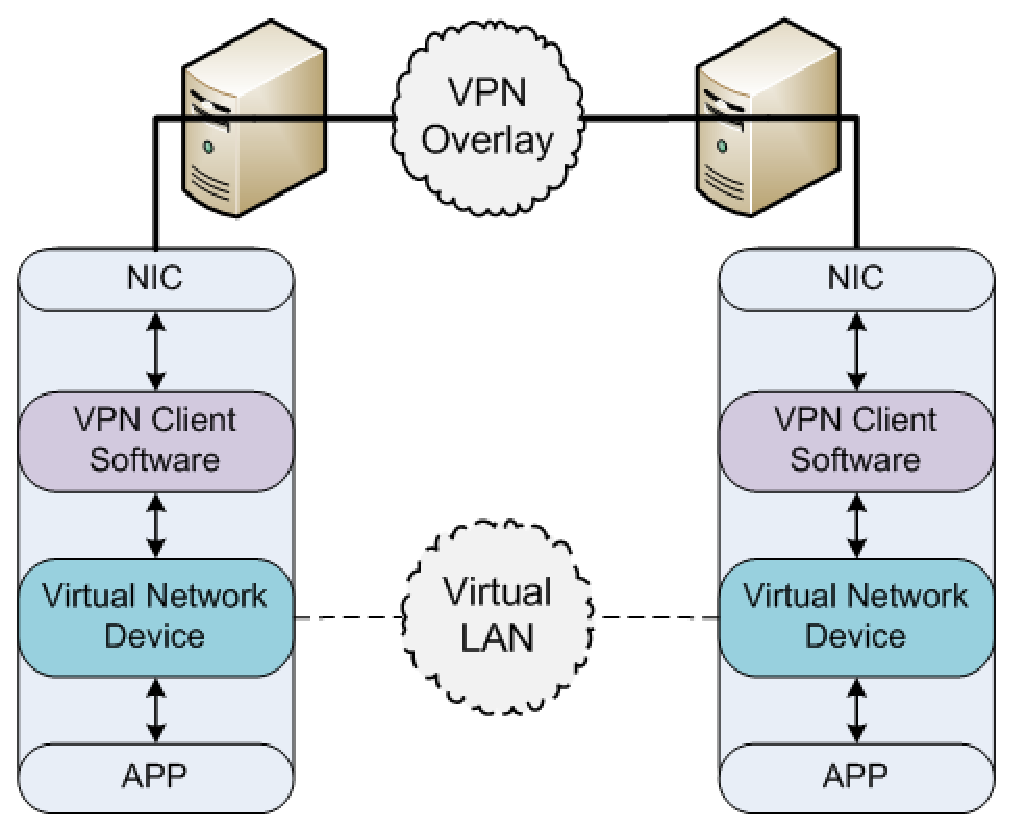
\epsfig{file=figs/vpn.png.eps, width=4in}
\caption[A typical VPN client]{A typical VPN client.  A VN device makes
application interaction with the VPN transparent.  Packets going to the VPN
destination are sent by routing rules to the VN device interfaced by the VPN
client.  The VPN client sends and receives packets from other VPN participants
via the hosts physical network device.}
\label{fig:vpn}
\end{figure}


%-----------------------------------------------------------------------%

% Includes appendices called into the appendix file(check the comments regarding editing your appendix in that file)
% The Editorial Office Requirements for the Table of Contents cause a significant problem 
%in Latex if there is only one Appendix. The Appendix is no longer labeled "A" in the TOC
%but has the word "APPENDIX" placed in front of the title of the Appendix. This can be done
%without issue IF nothing needs to be numbered by LaTeX in the Appendix. Unfortunately, most of the time
%something needs to be numbered in that single Appendix. For this reason we have included the IFTHENELSE switch
%found in this document and at the beginning of AppendixA. We assume that if you have any appendices, that you have more than one.
%So the default setting is noa = 2 (number of appendices = 2). Note: you don't need the actual number of appendices here
%1 or 2 are the only relevant numbers. You just make sure to input the Appendices you do have in this file.
%
%If, however, you DO only have one appendix change the line:
%
%\setcounter{noa}{2} to
%
%\setcounter{noa}{1}
%
%And comment (or delete) all of the input{AppendixB} commands except the first one.
%Then open the AppendixA.tex file and continue there.

%you can add/substract individual appendices through by using the /include{appendix'X'}
% and creating/deleting the appropriate files
\appendix %
\clearpage%
\newcounter{noa} % noa= no. of appendices ... set to 1 for 1 and more otherwise.
\setcounter{noa}{1} % ........................... CHANGE VALUE ONLY HERE
\ifthenelse{\value{noa} = 1}
%...................then
{}
%...................else
{\addtocontents{toc}{\protect\addvspace{10pt}\protect\noindent \protect APPENDIX}}
%...................
%If you have a single appendix, you need to change {\chapter*{APPENDIX: THIS IS THE FIRST APPENDIX}
%to {\chapter*{APPENDIX: YOUR APPENDIX TITLE HERE} if you have two or more appendices
%you need to change {\chapter{THIS IS THE FIRST APPENDIX}} to
%{\chapter{YOUR APPENDIX TITLE HERE}}
%
%If you make these changes correctly Latex will complain bitterly about the additions to the TOC
%but will make them correctly in a manner acceptable to the Editorial Office.

\ifthenelse{\value{noa} = 1}
%...................then
{\chapter*{APPENDIX: STRUCTURED OVERLAY BROADCAST}
\label{broadcast}
\addcontentsline{toc}{chapter}{APPENDIX: STRUCTURED OVERLAY BROADCAST}
\chaptermark{Appendix}
\markboth{Appendix}{Appendix}
\setcounter{chapter}{1}}
%...................else
{\chapter{STRUCTURED OVERLAY BROADCAST}
\label{broadcast}}
%...................

\begin{figure}[ht]
\centering
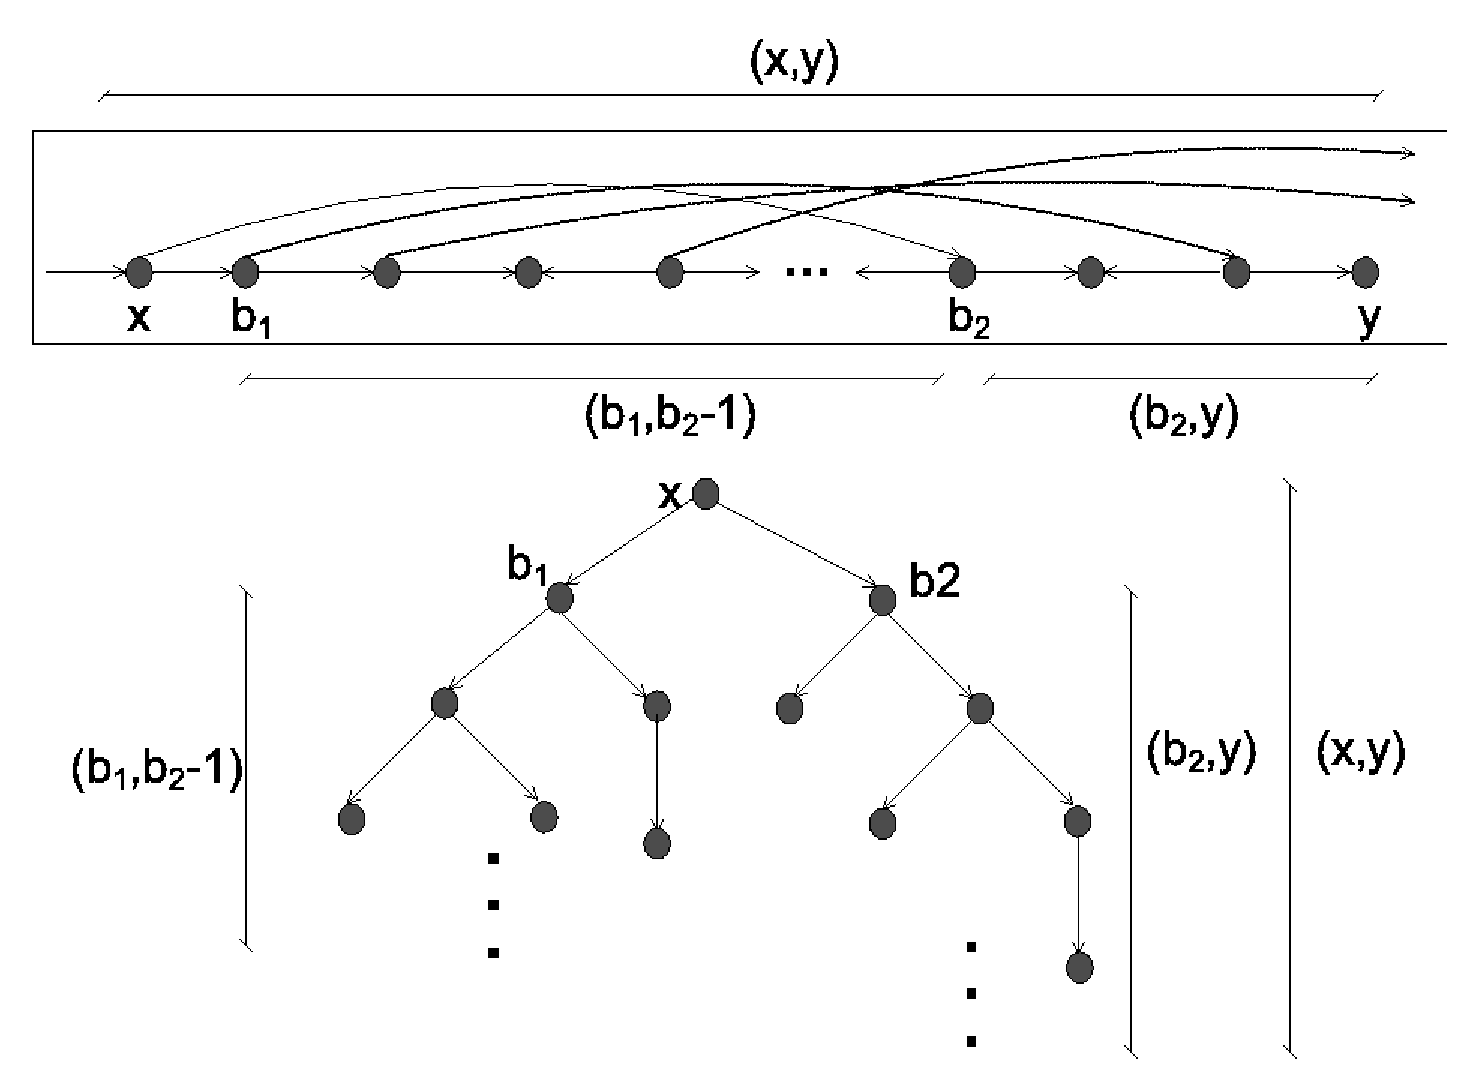
\includegraphics[width=4in]{figs/tree.eps}
\caption[Tree-based overlay broadcast]{Tree-based overlay broadcast}
\label{fig:tree}
\end{figure}  

Broadcast revocation can be used to address the deficiencies of DHT revocation.
As a topic of previous research works~\cite{broadcast, chord_broadcast},
structured overlays can be used without additional state to perform efficient
broadcasts from any point in the overlay to the entire overlay.  In these
papers, analysis and simulations have shown that the approach can be completed
in a network size of $n$ in $O(\log^2 n)$ time with $n$ messages.  The overlay
broadcast algorithm used in this paper provides a complete overlay broadcast in
$O(\log^2 n)$ time with $n$ messages.  When applied to Brunet, as illustrated
in Figure~\ref{fig:tree}, it utilizes the organization of a structured system
with a circular address space that requires peers be connected to those whose
node addresses are the closest to their own, features typical of
one-dimensional structured overlays including Chord~\cite{chord},
Pastry~\cite{pastry}, and Symphony.  Using such an organization, it is possible
to do perform a broadcast with no additional state.  To perform a broadcast,
each node performs the following recursive algorithm:

\begin{algorithmic}
\STATE {\bf BROADCAST(start, end, message)}:
  \STATE RECEIVE(message)
  \FOR{$i$ in length(connections)}
    \STATE n\_start $\gets$ ADDRESS(connections$[i]$)
    \IF {n\_start $\not\in$ $[$start, end$)$}
      \STATE continue
    \ENDIF
    \STATE n\_end $\gets$ ADDRESS(connections$[i+1]$)
    \IF {n\_end $\not\in$ $[$start, end$)$}
      \STATE n\_end $\gets$ end
    \ENDIF
    \STATE msg $\gets$ (BROADCAST, n\_start, n\_end, message)
    \STATE SEND(connections$[i]$, msg)
  \ENDFOR
\end{algorithmic}
with ``connections'' as a circular list of connections in non-decreasing order
from the perspective of the node performing the current recursive, broadcast
step.

In this algorithm, the broadcast initiator uses its own address as the start
and end, thus the broadcast will span the entire overlay after completing
recursive calls at each connected node.  A recursive end, ``n\_end'', must be
inside the region between ``start'' and ``end'', thus if the connection
following the current sending connection, ``connections$[i+1]$'', is not in
that region, it will only broadcast up to ``end'' and not the address specified
by that connection.  To summarize, the overlay is recursively partitioned
amongst the nodes at each hop in the broadcast.  By doing so, all nodes receive
the broadcast without receiving duplicate broadcast messages.

%If you have a single appendix, you need to change {\chapter*{APPENDIX: THIS IS THE FIRST APPENDIX}
%to {\chapter*{APPENDIX: YOUR APPENDIX TITLE HERE} if you have two or more appendices
%you need to change {\chapter{THIS IS THE FIRST APPENDIX}} to
%{\chapter{YOUR APPENDIX TITLE HERE}}
%
%If you make these changes correctly Latex will complain bitterly about the additions to the TOC
%but will make them correctly in a manner acceptable to the Editorial Office.

%\ifthenelse{\value{noa} = 1}
%...................then
%{\chapter*{APPENDIX: EVALUATION TOOLS}
%\label{evaluation_tools}
%\addcontentsline{toc}{chapter}{APPENDIX: EVALUATION TOOLS}
%\chaptermark{Appendix}
%\markboth{Appendix}{Appendix}
%\setcounter{chapter}{1}}
%...................else
{\chapter{EVALUATION TOOLS}
\label{evaluation_tools}}
%...................

Netperf~\cite{netperf} is used to estimate the latency and bandwidth of the
different VN models. The latency is measured by deploying Netperf in the
TCP\_RR mode, which measures the number of 1-byte request-receive transactions
that can be completed in a second. The bandwidth is estimated by running Netperf
in the TCP\_STREAM mode, which is a bulk transfer mode. It should be noted that
in situations where the link bandwidths were asymmetric, Netperf is deployed in
both directions.  Since both latency and bandwidth are dependent on the CPU
comparison, evaluations that include CPU utilization tasks require creating
a baseline first where only Netperf is the only active workload.

SPECjbb~\cite{specjbb} simulates a three-tier web application with all the
clients, the middle tier, and the database running on a single system in a
single address space (inside a JVM). On completion, the benchmark provides the
metric in terms of business of operations per second (bops). The bops score of
the system under test depends on both the CPU and the memory in the system, as
the entire database for the benchmark is held in memory. This benchmark
generates negligible disk activity and no network activity. 



%------------------------------------------%

% Make List of References (BibTeX implemented using the Natbib package)
% un-comment your preferred bibliography style and replace the
% bibliography file "sample" with the name of your .bib file
% REMEMBER!!! If you want un-numbered references comment the Natbib package with
% The numbered options in the packages.tex file and un-comment the package with the authoryear option
% See the included pdfs of the various styles to see the differences.
% The citation style differences are from the \citet{key} and \citep{key} commands
% More options are available; see the Natbib documentation for details


\bibliography{ufsampleETD}
% You can have more than one library of references
%------------------------------------------%

% Bio Sketch %
% Just type your bio in between the brackets
\biography{%

David Isaac Wolinsky was born on October 31, 1982.  He was blessed with an
awesome, Isaac Emmanuel, born November 30, 2009.  Beginning his studies in
August 2001 at the University of Florida, David obtained the following degrees
in electrical and computer engineering: Bachelor of Science in Spring 2005,
Master of Science in Spring 2007, and Doctorate of Philosophy in Summer 2011.
His advisor at the University of Florida was Professor Renato Figueiredo, whom
he began working with since the during the Spring of 2006 at the Advanced
Computing and Information Systems Lab.

His primary research focuses are network virtualization using structured P2P
(peer-to-peer) overlays and grid computing.  The networking research has been
realized in IPOP, a free (BSD - Berkeley Software Distribution licence))
network virtualization software.  Additionally, he has worked on enabling DHTs,
decentralized NAT (network address translation) traversal through relays,
software models for improved network virtualization, and autonomic virtual
networking stacks.  This work is a major contribution to his grid computing
research focus, Grid Appliance, which enables the creation of decentralized,
distributed grids using virtualized, physical, and cloud resources.  Going
forward, he expressed great interested in using these concepts in other
distributed systems such as sensor networks, social networks, cloud services,
or even web services.

During his free time, he enjoys time with my boy, running, playing basketball,
and occasionally playing video games.  At one point, he was ranked in the top
20 on the US East Warcraft III Free For All Ladder.  

}


%------------------------------------------%

\end{document}

%-------------------------------------------------------------------------------------------------------%
